\documentclass{style/llncs}

\usepackage{amsmath,amsfonts}
\usepackage{color}
\usepackage[usenames,dvipsnames,svgnames,table]{xcolor}
\usepackage[mathscr]{eucal}
\usepackage{thmtools}
\usepackage{graphicx}
\usepackage{caption}
\usepackage{subcaption}

\newcommand{\M}{\mathscr M}
\newcommand{\C}{\mathscr C}
\newcommand{\T}{\mathscr T}
\newcommand{\F}{\mathscr F}
\renewcommand{\P}{\mathscr P}
\newcommand{\K}{\mathscr K}
\newcommand{\X}{\mathscr X}
\newcommand{\B}{\mathbb B}
\newcommand{\D}{\Delta}
\newcommand{\N}{\mathbb N}
\newcommand{\tn}[1]{\textnormal{#1}}
\newcommand{\pair}[1]{\left\langle{#1}\right\rangle}
\newcommand{\concat}{\oplus}
\newcommand{\symb}[1]{\texttt{#1}}
\newcommand{\br}[1]{\overline{#1}}
\newcommand{\s}{S}
\newcommand{\dom}[1]{\mathop{\tn{dom}(#1)}}
\newcommand{\range}[1]{\mathop{\tn{range}(#1)}}

\newtheorem{conj}{Conjecture}

\let\doendproof\endproof
\renewcommand\endproof{~\hfill\qed\doendproof}

\newcommand{\p}{\,\text{.}}

\newcommand{\tuple}[1]{\left\langle{#1}\right\rangle}

\newcommand{\hide}[1]{}
\newcommand{\old}[1]{}

\newcommand{\sdr}[1]{\textcolor{blue}{\small #1\textsuperscript{[Steven]} }}
\newcommand{\pb}[1]{\textcolor{OliveGreen}{\small #1 \textsuperscript{[Peter]} }}

\newcommand{\argmin}{\mathop{\arg\min}}

% --- DELETE BEFORE SUBMISSIONS ---
\pagestyle{headings} 

\title{Three Problems for Sophistication}

\author{Peter Bloem and Steven de Rooij}

\institute{
  System and Network Engineering Group, \\University of Amsterdam, the Netherlands\\
  \email{uva@peterbloem.nl, steven.de.rooij@gmail.com}
}

\begin{document}
\maketitle

\begin{abstract}
Kolmogorov complexity measures the amount of information in data, but does not distinguish structure from noise. Kolmogorov's definition of the \emph{structure function} was the first attempt to measure only the structural information in data, by measuring the complexity of an objectively best model under two-part coding. Since then, many variations of this idea have been proposed, for which we use \emph{sophistication} as an umbrella term. We describe three fundamental problems with all existing proposals, showing each  to be \emph{unsound}. Consequently, we put forward the view that the problem is fundamental, it may be impossible to objectively quantify the sophistication.
\end{abstract}

\section{Introduction}
Komogorov complexity gives us a sound definition of the amount of information contained in a bitstring. There is, however, a nagging discrepancy between Kolmogorov complexity and what most people would consider complexity. For example, a sequence of a million coin flips will almost certainly have maximal Kolmogoroc complexity, even though there is nothing complex about flipping a lot of coins---it's just hard work. For this reason, many scholars have defined alternative complexity measures in the spirit of Kolmogorov complexity, aimed at quantifying not \emph{all} information in a binary string, but only the \emph{meaningful} information in the data. This tradition started with a lecture by Kolmogorov in Talinn in 1973, but many alternative definitions of meaningful information, or \emph{sophistication},\footnotemark were proposed. In this paper, we investigate three serious problems with these definitions, and show why they are unsatisfactory. We believe that the problems are fundamental, and provide arguments why such attempts to define sophistication must fail.

The Kolmogorov complexity of a binary string $x$, denoted $K(x)$, is (roughly) the length of the shortest computer program that will output $x$. This length depends on which programming language is used, but, as shown by a core result known as the Invariance Theorem, the language affects the result only by a constant, independent of $x$. This means that for sufficiently complex objects, the choice of programming language becomes irrelevant and Kolmogorov complexity becomes an \emph{objective} measure of the complexity of binary strings. We can see it as \emph{a property of the data}.

A robust definition of sophistication $S(x)$ in the spirit of Kolmogorov complexity should have similar robustness guarantees. We are interested in a measure satisfying the following requirements:

\begin{enumerate}
\item Since it measures information, $S(x)$ should count the bits required for an effective description of the structural properties of a binary string.
\item An analogue of invariance should hold for sophistication: at the very least, there should be strict limits on the degree to which a change in the programming language can affect the sophistication.
\item There should be no constant $c$ such that $S(x)\le c$ for every input $x$. If sophistication is bounded, then knowing its value under one programming language provides no constraints on its value under another language. Moreover, a bounded sophistication would be at odds with the intuition that there is no limit to the amount of structure that a binary string can exhibit.
\item Similarly, there should be no constant $c$ such that $K(x)-S(x)\le c$ for all $x$, because then sophistication would be equivalent to Kolmogorov complexity. 
\end{enumerate}
For most proposed definitions of sophistication, we can prove that they fail one or more of the conditions above. Vit\'anyi's definition \cite{vitanyi2004meaningful} is the one exception that we cannot \emph{prove} to conflict with our requirements, but we can show that only strings that require an enormous amount of processing to construct, yield a large sophistication.

A valid definition of $S$ must contend with the following issues. First, the representation of the model is crucial. This is particularly important to those treatments that `open up' the definition of $K$, to consider the representation that witnesses the Kolmogorov complexity. In Section~\ref{section:indices}, we discuss the \emph{nickname problem}: the sophistication becomes highly dependent on the chosen programming language, unless it can represent functions with maximum efficiency. 

The second issue is that of \emph{overfitting}, which we consider in Section~\ref{section:overfitting}. Overfitting is a common problem in the statistical literature, that refers to the tendency of model selection to choose a very complex model that provides a very good fit to the observed data, but does not generalise well to unseen data. For example, in a polynomial regression setting, a polynomial of sufficiently high order can always cover all data points. However, if the data was sampled from a straight line, with a small amount of noise, such a polynomial would be far too complex: it would encode all noise inside the model. The same can occur for the sophistication. We somehow need to make sure that the two-part representation that determines the sophistication does not store noise in the ``structure'' part of the code. In statistics, this is typically addressed by penalising complex models. In sophistication, however, such penalties tend to break the balance between structural information and noise, and lead to the opposite problem: underfitting.

Underfitting (Section~\ref{section:underfitting}) occurs when the selected model is simple, but fails to represent some of the structure present in the data. This is a problem for sophistication because the considered models can be so powerful. In particular, in any programming language, there are programs that implement an interpreter for \emph{another} language. Such \emph{universal models} can be described in a constant amount of bits, and  represent the data with an input of the length of the Kolmogorov complexity, essentially encoding all information as noise. If complex models are penalized, then the problem becomes to make sure that universal models are not \emph{always} preferred for complex data. The usual workaround is to restrict the set of allowed models to exclude the universal ones. For example, the model class may be restricted to the set of all total recursive functions. While excludes universal models, it is questionable whether it adequately solves the problem of underfitting in general.

Finally, in the discussion in Section~\ref{section:conclusion} we argue that while two-part coding can yield useful insights into the structure of the data and allows us to identify some models as poor representations, it is probably not possible to uniquely separate structure from noise and identify a \emph{single} model as ``best'': in general many models, of vastly different complexities, may be reasonable representations. Rather than doggedly trying to ``fix'' this property of algorithmic statistics, we propose embracing the idea that the data allows for multiple equivalent interpretations, and that there is no such thing as sophistication.

\subsection{Related work}
The idea of separating structure from noise originated with Kolmogorov's \emph{structure function} \cite{cover1985kolmogorov}. In this theory, the data is described as finite set together with an index in the set. The complexity of the set determines the sophistication. This approach was discussed more extensively, and generalised in \cite{vereshchagin2004kolmogorov,gacs2001algorithmic}. 

Koppel \cite{koppelSoph1988,koppel1991almost} also built on the structure function work to define a measure of the meaningful information in a binary string, coining \emph{sophistication}, the name we adopt in this paper. 

In 1996 Gell-Mann and Lloyd introduced \emph{effective complexity} \cite{gellmann1996information}. Working from the perspective of statistical mechanics, they arrived (independently, it seems) at a notion that fits the mold of sophistication.


Antunes et al. \cite{antunes2009sophistication} note that the constant cutoff used by Koppel is a source of instability, a result in the spirit of this paper. They propose a different definition called \emph{coarse sophistication}. As we shall see, this version behaves very differently from regular sophistication, and is closer to computational depth. Vereshchagin \cite{vereshchagin2013algorithmic}, working in the finite set setting,  suggests additional restrictions on models that are allowed to determine the sophistication, in hopes of curbing the instability issue. Adriaans' \emph{Facticity}, introduced in 2012\cite{adriaans2012facticity}, relaxes the model class to include all partial recursive functions. Adriaans also identifies the nickname problem discussed in Section~\ref{section:indices}.

\section{Preliminaries}
Let $\B = \{0,1\}^*$. We deal with partial computable functions $\phi: \B \to \B$, which we will also call \emph{models}. A function is called \emph{prefix} if its domain, $\dom{f} = \{y : f(y) \neq \infty\}$ is a prefix free set, i.e. no string in $\dom{f}$ is a prefix of another. A function $f$ is \emph{total} if $\dom{f} = \B$.

A \emph{numbering} is an enumeration of of the partial computable functions, denoted as $\psi_1, \psi_2, \ldots$ or simply $\psi$. We fix one canonical effective numbering $\phi$. We call a numbering $\psi$ \emph{acceptable} if there exist total, computable functions $a, b: \N \to \N$ with $\forall: i$, $\phi_i = \psi_{b(i)}$ and  $\psi_i = \phi_{a(i)}$.

A \emph{model class} is a set of model indices. We distinguish four important model classes: 
\begin{enumerate}
\item $\C=\N$, the indices of all partial computable functions
\item $\T=\{i:\tn{$\phi_i$ is total}\}$. Note that $\T$ is not enumerable.
\item $\K$ is an enumerable set such that $\{\phi_i:i\in\K\}$ is the set of all partial computable prefix functions
\item $\F$ is an enumerable set such that $\{\phi_i:i\in\F\}$ contains a uniform code for every finite set. A uniform code for a finite set $S$ is a total computable surjective function $f:\{0,1\}^{\lceil|S|\rceil}\to S$.
\end{enumerate}

We sometimes need to map binary strings to a prefix-free set. We denote by $\bar x$ the prefix-encoded representation for $x$. We require that the mapping satisfies $|\bar{x}| = |x|+O(\log(|x|)$ (see eg. \cite[Section~1.4]{li1993introduction}). To simplify notation, we will sometimes conflate natural numbers and binary strings, implicitly using the ordering $(0, \epsilon)$, $(1, 0)$, $(2, 1)$, $(3, 00)$, $(4, 01)$, \ldots

Now define the Kolmogorov complexity of a binary string $x$, with respect to a model class $\M$ and a numbering $\psi$, as follows:
\[
C^{\M,\psi}(x)=\min\{\bar\imath y:\psi_i(y)=x,i\in\M\}.
\]
The model class $\C$ gives us the plain Kolmogorov complexity and the $\K$ gives us the prefix-free Kolmogorov complexity. The complexity is invariant to the numbering for these model classes, so we may omit it from the superscript.

A pair $(i,y)$ is a \emph{representation} for $x$ if $\phi_i(y)=x$.

\begin{figure*}[tb]
  \hspace{-0.9cm}
  \begin{subfigure}[b]{0.55\textwidth}    
     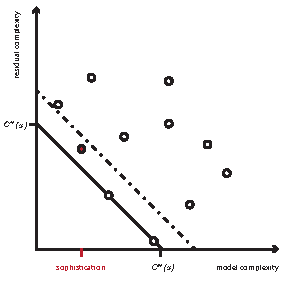
\includegraphics[width=\textwidth]{./img/sophistication.pdf}
      \label{figure:sophistication}
  \end{subfigure}
  \begin{subfigure}[b]{0.55\textwidth} 
     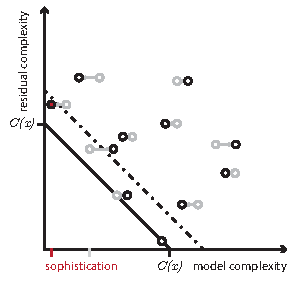
\includegraphics[width=\textwidth]{./img/sophistication-jump.pdf}
      \label{figure:sophistication-jump}
  \end{subfigure}
  
  \caption{\small (left) A schematic representation of the idea of sophistication. We can represent the data $x$ in two parts: by describing first, a model, and then the residual information required to specify the data given the model. The smallest possible effective description, denoted by a black diagonal, is $C^\M(x)$. We accept all representation that come within a given \emph{slack} of this optimum, represented by a dashed line. The size of the smallest model within the slack is the sophistication of the data. (right) The same image, after a constant perturbation  in te model complexity caused by a change in numbering.}
  \label{fig:diagram}
\end{figure*}

\section{Inefficient indices}
\label{section:indices}
As mentioned in the introduction, the definition of sophistication is sometimes obtained by opening up the definition of Kolmogorov complexity, and measuring the length of the index part of that two-part code. We call such a sophistication \emph{index sophistication}. Examples are Koppel and Atlan's works \cite{koppelSoph1988,koppel1991almost},  and several of its variants \cite{antunes2009sophistication,antunes2013sophistication}. 

In these works, no constraints are placed on the used numbering. This makes these approaches vulnerable to the so-called \emph{nickname problem}: the number of bits required to specify a model becomes very dependent on the numbering. This problem is severe: any index sophistication without requirements on the numbering is either bounded, or not invariant:

\begin{lemma}
Let $s^\psi$ denote any index sophistication with respect to numbering $\psi$.
There are acceptable numberings $\psi$ and $\xi$ such that for all $x$:
\[|s^\xi(x) - s^\psi(x)|\geq \frac{1}{2}\min\{s^\psi(x),s^\xi(x)\}\p\]
\end{lemma}

To prove this, we use numberings that are deliberately extremely inefficient:

\begin{proof}
Let $s_i$ be the binary string consisting of $2^{i}$ zeroes followed by a one.

Define $\psi$ and $\xi$ by
\[
\psi_j(x) = \begin{cases}
	\phi_i(x) \;\text{if}\; j = s_{2i}\\
	\infty\;\text{otherwise}
\end{cases}\,\,\,
\xi_j(x) = 
\begin{cases}
	\phi_i(x) \;\text{if}\; j = s_{2i+1} \\
	\infty \;\text{otherwise}\p
\end{cases}
\]
Choose any $x$ and assume w.l.o.g. that $s^\psi(x)\le s^\xi(x)$. By construction of $\psi$ and $\xi$ we have $2s_\psi(x)  \leq s_\xi(x)$ from which the result follows.
\end{proof}
While the invariance theorem expresses that inefficient indices do not affect Kolmogorov complexity too much, this robustness property does \emph{not} carry over to index sophistication. In other words, the length of a model index does \emph{not} represent its complexity.

In order to obtain a reasonable and robust measure of model complexity, we  extend the definition of Kolmogorov complexity to functions:

\begin{definition}[\cite{grunwald2004shannon,vitanyi2004meaningful}]
The complexity of a computable function is defined by \label{definition:model-complexity}
\[
C^{\M,\psi}(f) = \min\{C^{\M,\psi}(i):\phi_i=f\}\p
\]
\end{definition}
We show in the appendix (Lemma~\ref{lemma:invariance}) that this definition is invariant, so that the Kolmogorov complexity is an objective property of a function, as it is of a binary string. There are two ways to use this notion of model complexity for more robust attempts to define sophistication. Confusingly, both approaches are used in the literature.
\begin{enumerate}
  \item We maintain that the representation witnessing the Kolmogorov complexity determines the sophistication, but impose the additional constraint that an efficient acceptable numbering is used. We construct such an efficient index, called a \emph{faithful} index, below. This is the approach taken by Adriaans \cite{adriaans2012facticity}.
  \item On the other hand, rather than distinguishing the two components of the code \emph{within} the definition of Kolmogorov complexity, we can also use $K$ to measure the complexity of the \emph{model} (as in Definition~\ref{definition:model-complexity}), which is then the first part of a two-part code describing the data. With this approach, the total code length is $K(\phi_i)+|y|$, with $\phi_i(y)=x$. In this approach, we can construct everything on the basis of a single acceptable numbering, without additional constraints. This approach is used in  \cite{cover1985kolmogorov,gacs2001algorithmic,vitanyi2004meaningful,gellmann1996information}.
\end{enumerate}
We first construct an efficient numbering: we will call a numbering $\psi$ \emph{faithful} if for all $i$ there is a $j$ such that $\psi_i=\psi_j$ and $|j|\le C^{\C}(\psi_j)+c$, for some constant $c$. This definition is a refinement of \cite[Definition~10]{adriaans2012facticity}. 

\begin{lemma}
There exist faithful acceptable numberings.
\end{lemma}
Unfortunately, even with a faithful numbering, we can fail. The Kolmogorov complexity uses representations of the form $\bar\imath y$, where the bar denotes some straightforward prefix encoding to delimit the model description $i$ from its input $y$. If we define a second prefix encoding $\tilde{\imath}$, which is always better than our default by some slowly growing term, such as $O(\log\log\log i)$, we can define a second representation $\bar u \tilde \imath y$, which takes a constant amount of bits $|\bar u|$ to switch to a different universal model, but gains more than a constant, for sufficiently complex strings, because a different prefix function is used. Ultimately, $u$ would always be chosen as a model for sufficiently complex $x$.

Can we make our prefix encoding so efficient that no other encoding can undercut it by more than a constant amount? One self-delimiting description of $\phi_i$ is the one used in $C^\K(\phi_i)$. By definition, this is the smallest effective, self-delimiting description of $\phi_i$. Let $i^*$ be a the shortest self-delimiting program for $\phi_i$. If our prefix function is less efficient than $C^\K(x)$ by an unbounded amount, the effective representation $i^*y$ will always beat $\bar\imath y$ for complex enough data. We conjecture that no computable prefix encoding function can avoid this issue:
\begin{conjecture}
For any partial computable prefix codelength function $L$, the function $\min\{L(i)-C^\K(i):i\ge i_0\}$
is unbounded in $i_0$.
\end{conjecture}
The following lemma shows that for all index sophistications using an inefficient prefix encoding will fail. This includes \cite{adriaans2012facticity}.
\begin{restatable}{lemma}{ineffprefix}
Assume $\phi$ is faithful and define the index sophistication $s^c(x)=\min\{|\bar\imath|:C^{\{i\}}(x)\le C^{\C}(x)+c\}$.
If $\min\{i\ge i_0:|\bar\imath|-C^\K(i)\}$ is an unbounded function of $i_0$, then $s^c$ is bounded.\label{lemma:prefix-inefficiency}
\end{restatable}

If our conjecture is correct, the index sophistication is always bounded. The only way to avoid the problem is to use a the self-delimiting program of length $C^\K(x)$ to describe the model. Any inefficieny in the model description, and a second represention using a universal model with a more efficient model description will win, causing a bounded sophistication.

For this reason we will using the following definition of sophistication in the remainder of this article: 
\begin{equation}\label{eq:soph}
S^{\M,\psi,c}(x)=\min\left\{C^\K(\phi_i):i\in\M,C^{\{i\},\psi}(x)\le C^{\M,\psi}(x)+c\right\}.
\end{equation}

\section{Balancing under- and overfitting}
\label{section:balance}

In the previous section, we saw the first glimpse of how delicate the internal balance in sophistication is. If the description of the model $m$ is less efficient than $C^\K(m)$ by anything more than a constant, representations with a bounded model size will always win out in the limit. 
In light of this balance issues, the most natural definition of sophistication is $S^{\K,\psi,c}$. In this setting, we know that there always exist candidate models---those models $i$ with $i \in \K$ and $C^{i}(x) \leq C^\K(x) + c$---for which al information except a constant amount is stored in the data, and candidates for which all information is stored in the model. This tells us that $S^\K$ is \emph{balanced}: there is no inefficiency in the representation forcing information in or out of the model.
The flipside of having a balanced sophistication is that invariance is easy to show. We will show that there are numberings for which the universal models always determine the $S^\K$ and numberings for which the singletons always determine $S^\K$. 
	The following lemma generalizes the principle: 
\begin{restatable}{lemma}{coolone}
\label{lemma:thecoolone}
  Let $\psi$ be any acceptable enumeration of the partial recursive functions.
  Let $\M$ be any model class, let $\X$ be any set of binary sequences and let $D:\B\to\N$ be a computable decoding function with a prefix-free domain that maps function descriptions to their indices in $\psi$, i.e. if $f=\psi_{D(p)}$ then $p$ is a $D$-description of $f$. Let $\M'=\{\psi_i:i\in\tn{range}(D)\}$. Further assume there is a constant $c$ such that:\\
\-\hspace{1cm}(1)$\forall_{f\in\M'}:\min\{|p|:\psi_{D(p)}=f\}\le K^\psi(f)+c$\\
\-\hspace{1cm}(2)$\forall_{x\in\X}:L^{\M',\psi}(x)-L^{\M,\psi}(x)\le c$.\\
Then there is an enumeration $\phi$ of the partial recursive functions such that $S^\phi_{\M}(x) = |\bar 0|+S^\psi_{\M'}(x)$ for all $x\in\X$.
\end{restatable}

This is a technical lemma, due to the double effect of the numbering, which occurs in both the definition of model complexity and the definition of data complexity. The \emph{idea} behind the lemma, however, is simple. Given a subset $\M'$ of the model class, we can choose the numbering so that representations use a model in $\M'$ perform an arbitrary constant better than all other models. This lets us effectively `push' all other models out of the candidate set, so that the sophistication is determined by a model in $\M'$.- can make it equal to $C^K$

This allows us to ensure that for some numberings, the unversal model always determines the sophistication, making is bounded:

\begin{restatable}[underfitting]{lemma}{underfitting}
Let $\M$ be a model class containing a universal model $u$, with the property that $\exists c \forall m \in \M : L^u(x) \leq L^m(x) + c \p$. Then, there exist numberings such that $\s^\M$ is bounded.
\end{restatable}
For other numberings, the singletons determine the sophistication, making it equal to the complexity:
\begin{restatable}[Overfitting]{lemma}{overfitting}
Let $\M \subseteq \K$ be a model class where for every $x\in\X$ there is a singleton model $f\in\M$ with $f(\epsilon)=x$. Then there is an enumeration $\phi$ of the prefix partial recursive functions, and a constant $c$, such that
\[
K(x)-S^{\M,\phi}(x)\le c
\]
for all $x\in\X$.
\end{restatable}
This shows that the price we pay for balance is absolute invariance. All information can be seen as structure of noise, depending on the numbering. To avoid these issues, existing proposals upset the balance to exclude, or penalize at least the singleton models and the universal models.
 
\subsection{Overfitting}

The existing proposals that do not avoid overfitting as the structure function \cite{cover1985kolmogorov}, the sophistication as defined in \cite{mota2013sophistication}, the miinimal sufficient statistic \cite{gacs2001algorithmic} and Vereshchagin's strongly  sufficient statistic \cite{vereshchagin2013algorithmic}. It may be argued that the constant determining the candidates should be allowed to depend on the numbering, but this dependence has not been mentioned in the literature and there is no clear way to determine what such a constant should be, on the basis of a given numbering. 

In traditional statistics, overfitting is often addressed by imposing a penalty on complex models. As we have seen, a strong penalty, such as the one imposed by an inefficient prefix encoding of the model, will immediately cause underfitting. A more subtle approach is to use $C$ as a model class, allowing representations that are not self-delimiting. This eliminates at least the singletons, as placing all information in the model automatically creates a self delimiting representation. Self delimiting representations are longer than plain representations, and this gap is unbounded \cite[Section~4.5.5]{vitanyi2004meaningful}, which tells us that singletons will be candidates for only finitely many strings. This approach is taken by Vit\'anyi \cite{vitanyi2004meaningful} and by Adriaans \cite{adriaans2012facticity}. 

\subsection{Underfitting}

Underfitting is a widely acknowledged problem, and almost all proposals avoid it by limiting the class of allowed models, to exclude universal models. Does this make the sophistication unbounded? The following theorem shows that it does.

\begin{restatable}{theorem}{dogfood}
There are infinitely many $x$ with $\s^{\F,\phi,c}(x) \geq C^{\K}(x)/5$ and $\s^{\T,\phi,c}(x) \geq C^{\K}(x)/6$. 
\end{restatable} 

But clearly, this only exacerbates the overfitting problem. Only one model class eliminates both the singletons and the unversal model: $S^\T(x)$. The only proposal that uses an efficient model representation, excludes the universal models and excludes the singletons is Vit\'anyi's \cite{vitanyi2004meaningful}. While this invalidates straightforward proofs of boundedness, there is no suggestion that $S^\T(x)$ is actually invariant.

While under $S^{\T, \phi, c}(x)$ there are clearly string with high sophistication, these may not conform to the original intuition that motivated sophistication. To show this, we require the concept of depth:

\begin{definition}[Depth\cite{bennett1988logical,antunes2006computational}]\belowdisplayskip=-12pt
Let $U$ be some universal Turing machine, so that $U(\bar\imath y) = \phi_i(y)$. Let $U^t$ be a simulation of this machine, which is allowed to run for at most $t$ steps, and returns $0$ if it has not yet finished at that point. Let $C^t_\M(x) = \min\{|\bar\imath y| : U^t(\bar\imath y) = x, \phi_i \in \M\}$.

The \emph{$c$-depth} $d^\M_c(x)$ of a string is $d^\M_c(x) = \min \left\{t : C^\M_t(x) - C^\M(x) \leq c \right\}$.
\end{definition}

Deep strings are those that can only be optimally compressed with a great investment of time. We note that it is exceedingly unlikely that a deep string is sampled from a shallow distribution \cite{bloem2014safe,bennett1988logical}.
 
\begin{restatable}{theorem}{depth}
Let $A(n)$ be the single-argument Ackermann function and $c$ some arbitrary constant. There are numberings such that for all strings with depth $d^\C_c(x) \leq A(C(x))$, $\s^\T(x)$, $s^\P(x)$ and $\s^\F$ are bounded.
\end{restatable}
\noindent This shows that while high-sophistication strings exist, they do not behave as expected. Consider a string that is typical for a low-depth model, say some high-complexity Markov chain. Under sophistication, no matter how complex the markov chain, the sophistication would stay the same. Any structure that is simple enough to be exploited within the time bound of the Ackermann function (or some other fast-growing, simply stated bound) will be counted as noise. Only structure that is so deep that if we used it to compress $x$ we could never hope to decompress it within the lifetime of the universe, would count towards sophistication. 
This clearly contradicts the motivating principle of sophistication, which is to capture the number of bits required to express \emph{all} regularity in the data. 
What makes a string high-sophistication is not the fact that it has a great deal of structure, but the fact that it can be compressed far better with partial functions than with total. That is, it is non-typical for the model class $\T$. This suggests that the `non-stochastic' property of strings with high sophistication \cite{shen1983concept,vereshchagin2004kolmogorov} says more about depth and totality than it does about structure and noise.

The relation between sophistication, depth and absolutely non-stochastic strings was also investigated in \cite{antunes2013sophistication}.

\section{Discussion}
\label{section:conclusion}

So why should we consider this intuition reasonable at all? The first assumption of sophistication is that high compressibility and pure randomness are objectively `uninteresting'. A more sophisticated signal, such as a television broadcast must contain, in some objective sense, more meaningful information. Whether this intuition seems reasonable likely differs per person \sdr{weak}, but sophistication goes one step further: it also suggests that we can objectively separate the information in a string into random and structured. \sdr{I think here we should sell the intuition better before we tear it down.}

To see whether this intuition is valid; imagine that we sample from the universal distribution by feeding random bits to a universal Turing machine, machine $u$ in the $\phi$-enumeration. If this UTM is constructed in the conventional manner, the initial bits will determine the index of a partial computable function $i$, and the rest will be the input $y$ to that machine. What is the characteristic model of the resulting data? Certainly, if we have to judge based only on the data we cannot exclude the possibility that the data was sampled from $\phi_u$: after all, it was.  On the other hand, neither can we exclude the possibility that it was generated by $\phi_i$, as again, it was! 

Although sampling perspectives are discouraged by proponents of algorithmic statistics, this statistical sanity check illustrates why it seems unjustified to assume that, based on only the data, all but one model can always be disqualified. \sdr{Hier stond: There is no reason to assume that a string with high sophistication was sampled from a complex model, so how can a complex model be intrinsic to the data? \footnotemark}

\footnotetext{Note that computational depth does not have this problem. Only deep sources produce deep strings.}

Consider the following metaphor. We are given a bitstring which can be read as a bitmap image of the painting \emph{Impression of a Sunrise}. The candidate set for this string contains various models from very generic to very specific. The theory behind sophistication suggests that we can choose one of these as the objective, intrinsic model of the data. Different models say different things: the universal models says that it is `something computable'. A more specific model might say that it is `an image'. Even more specific would be a painting, a Monet, or specifically the painting Impression of a sunrise. These are the models we imagine we may find in the candidate set. Can we say that the data is intrinsically more of an image than a painting? More of a Monet than a painting? We see no intuitive reason why such a distinction should be possible without making any further assumptions.

Of course, \sdr{Actually this is not trivial at all} Kolmogorov complexity allows us to say that it is unlikely to be a Jackson Pollock, or a piece of music. And, if we were to get a second sample from the same source, we \emph{could} answer the question: we would receive either the same painting again, or perhaps another Monet. But, a single sample does not give us enough evidence to choose a single model. \sdr{Volgende zin weer zwak, de metafoor wordt backed up door ons voorbeeld hierboven dus is behoorlijk hard} Ultimately, this is just a metaphor, but since the notion of sophistication is driven by intuition, we feel that an intuition to the contrary should serve to sharpen the debate.

For this reason, we take a skeptical view of sophistication. We can offer the following insight, to back up our skepticism. As we have seen, candidates within a constant of the optimal representation can occur all over the spectrum, from small to large models. A small change in construction, such as a different acceptable numbering, or a change in threshold function, can arbitrarily push models into or out of the candidate set. Whereas in Kolmogorov complexity, constant changes have constant effects on the outcome, here constant changes can cause large changes in the outcome. \sdr{Not sufficiently clear} While no authors have touched on the issue of invariance, it is related to the issue of instability \cite{antunes2013sophistication,vereshchagin2013algorithmic}. We consider invariance the first criterion by which any proposal must be judged, with the burden of proof resting with the proposer, rather than the critic.

Finally, we note that the use of total functions has a very subtle effect on the discussion surrounding sophistication. Since the total functions are not enumerable, the value of the sophistication relies strongly on the difference between the Kolmogorov complexity and the Kolmogorov complexity restricted to total functions. This gap is exceedingly difficult to capture, because the total functions cannot be enumerated. This is dangerous: if such definitions cannot be proved wrong or right, they will stand as the ad-hoc official view, while the restrictions used to elude proofs of incorrectness make them very difficult to build on. This creates an artificial dead end for a very valuable area of research. 


\sdr{Something about what is useful about the theory}
\sdr{A picture of the structure function (perhaps sooner as well)}
\sdr{This has become a discussion section. It does not recap. That's a bit unusual.}

\section{Conclusion}
As we have seen, the idea behind sophistication has a rich history. It has been proposed many times, by many different authors. This tells us two things. First, there is a strong intuition behind sophistication, shared by many respected authors, and second, it is not easy to get the definition exactly right.


\subsubsection*{\ackname}

This publication was supported by the Dutch national program COMMIT and by  the Netherlands eScience center.

\bibliographystyle{plain}
\bibliography{facticity}

\appendix

\section{Proofs and further discussion}

\subsection{Invariance of function complexity}

\begin{lemma}[Invariance of function complexity]
Let $\phi$ and $\psi$ be any two acceptable numberings. There exists a constant $c$ such that $\left| K_\phi(f) - K_\psi(f)\right | \leq c$ for all $f$. \label{lemma:invariance}
\end{lemma}
\begin{proof}
Let $g(i)$ be the function such that $\psi_i=\phi_{g(i)}$.
\begin{align*}
K_\phi(f) &= \min\left\{ K_\phi(i) : \phi_i= f\right\} 
\geq \min\left\{ K_\psi(i) : \phi_i= f\right\} - c\\
&= \min\left\{ K_\psi(i) : \psi_{g(i)}= f\right\} - c
\geq \min\left\{ K_\psi(i) : \psi_i= f\right\} - c' = K_\psi(f).
\end{align*}
The opposite inequality can be achieved by reversing $\phi$ and $\psi$. 
\end{proof}
This lemma shows that the complexity of a function does not depend on the choice of
enumeration by more than a constant term.

\begin{lemma}
  There is a faithful acceptable numbering.\label{lemma:faithful-numberings}
\end{lemma}
\begin{proof}
Let $\tn{div} \in \N$ be an index such that $\phi_{\tn{div}}(y)=\infty$ for all $y$. Define
  \[\psi_q=\begin{cases}
    \phi_{\phi_i(p)}&\tn{if $q$ can be written as $\bar\imath p$ and $\phi_i(p)<\infty$,}\\
    \phi_{i_\tn{div}}&\tn{otherwise.}\end{cases}
  \]
  To show that $\psi$ is faithful, pick any function $f$. Then
\[\begin{split}
C(f)&=\min\{C(i):\phi_i=f\} =\min\{\min\{|\bar a b|:\phi_a(b)=i\}:\phi_i=f\} \\
& =\min\{|\bar a b|:\phi_{\phi_a(b)}=f\}
 =\min\{|\bar a b|:\psi_{\bar a b}=f\}.
\end{split}\]
This shows there is a sufficiently small $\psi$ index.

To show that $\psi$ is acceptable, let $\phi_j$ denote the identity
function. Then a $\phi$-index $i$ can be mapped to a $\psi$-index
using the computable function $r(i)=\bar\jmath i$, so that
$\psi_{r(i)}(y)=\psi_{\bar\jmath i}(y)=\phi_i(y)$. For the reverse,
define $\phi_v(\bar\imath p, y)=\phi_{\phi_i(p)}(y)$. For fixed
$\bar\imath p$, the 
$s^n_m$-theorem \cite{kleene193notation} states that we can compute the $h$
such that $\phi_h(y)=\phi_v(\bar\imath p,y)$. Let $h(\bar\imath p)$
denote this index as a function of the program; further define
$h(q)=\tn{div}$ if $q$ cannot be expressed as $\bar\imath p$. By
construction $h$ is total and computable. To check that the mapping
returns the correct function, rewrite $\phi_{h(\bar\imath
  p)}(y)=\phi_v(\bar\imath p,y)=\phi_{\phi_i(p)}(y)=\psi_{\bar\imath p}(y)$.
\end{proof}

\subsection{Inefficient indices}
\label{section:appendix-inefficient-indices}

\ineffprefix*
\begin{proof}
Let $\bar\imath y$ be any two-part representation for the data $x$, i.e. $\phi_i(y)=x$. Then construct an alternative two-part representation $\bar vi^* y$, where $i^*$ is the shortest $\psi_u$-program for $i$ such that $\phi_v(i^* y)=\phi_{\psi_u(i^*)}(y) = \phi_i(y)=x$. We compare the lengths of these two representations. Note that $|i^*|=K^\psi(i)$. Therefore,
\[
|\bar\imath p|-|\bar v i^* y| = |\bar\imath|-|\bar v| - |i^*| = |\bar\imath|-|\bar v|-K(i).
\]
By assumption there must be an $i_0$ such that the above expression is positive for all $i>i_0$. From this $i_0$ onwards, the second representation (using $v$) will have a shorter code length, so $\bar\imath p$ cannot achieve the minimum in the definition of the sophistication. Consequently, the sophistication is bounded by $\s(x)<|\overline{\imath_0}|$ for all $x$. 
\end{proof}

\subsection{Boosting a model class by manipulating the numbering}

\coolone*

\begin{proof}
We define the numbering $\phi$ as follows:
\[\begin{cases}
\phi_0(p) = 1^r 0 D(p) \\
\phi_{1^r0i}(p) = \psi_i(p) \\
\phi_j(\cdot) = \infty &\text{if $j$ contains no zeroes.}
\end{cases}\]
We will show that under the $\phi$-enumeration, the best representation for $x$ using a model $f\in\M'$ is always better than the best representation using some $f\not\in\M'$.

First suppose $f\in\M'$. Then
\begin{align*}
K^\phi(f) &=\min\{|\bar\jmath q|:\phi_{\phi_j(q)}=f\}
\leq\min\{|\bar0 q|:\phi_{\phi_0(q)}=f\} \\ 
&=\min\{|\bar0 q|:\phi_{1^r0 D(q)}=f\}  
=|\bar 0|+\min\{|q|:\psi_{D(q)}=f\}
\leq K^\psi(f)+c+|\bar 0|,
\end{align*}
where the last inequality uses the first assumption.

Now assume that the best model $f$ for $x$ is not in $\M'$. 
Let $i$ be the index of $f$ with the shortest description, i.e. it achieves the minimum in $K^\phi(f)=\min\{K^\phi(i):\phi_i=f\}$.
There are two possibilities. Either $i=0$, in which case we have $K^\phi(f)\ge r$ because $\phi_0$ cannot output zero and all other $\phi$-programs are at least $r$ bits long.

Otherwise, we can bound
\begin{align*}
K^\phi(f)&=K^\phi(i)=K^\phi(1^r0j)\\
&\ge K^\phi(j)-c' \ge K^\psi(j)+r+1-c'\\
&=K^\psi(f)+r+1-c'.
\end{align*}
Now choose $r=c''+\max\{K^\psi(\phi_0),c'-1\}$. Then substitution yields, for both cases, 
$K^\phi(f)\ge c''+K^\psi(f)$.

Combining the inequalities above, for any model $g\not\in\M'$, there is a model $f\in\M$ such that
\[\begin{split}
K^\phi(g)+C^g(x) &\ge K^\psi(g)+C^g(x)+c''\\
&\ge K^\phi(f)+C^f(x) -2c+c'' -|\bar0|.
\end{split}\]

By choosing $c''$ sufficiently large, we can ensure that the best representation is in $\M'$ for all $x\in\X$, which completes the proof.
\end{proof}



\subsection{Overfitting}

\overfitting*

\begin{proof}
Let $\psi$ \sdr{This should probably be $\phi$} be any default enumeration of the partial recursive prefix functions. Note that since $f$ is a prefix function, if $f$ is defined for input $\epsilon$ then it cannot be defined for any other input. Pick $f,x$ with $f(\epsilon)=x$. Note that $x$ can be computed from $f$ and a fixed program, so there is a $c$ such that $K(x)\le K(f)+c$. Vice versa, given any $x$ we can construct an index of $f$, since $\psi$ is an acceptable numbering. Therefore $|K(f)-K(x)|\le c$.

We now define a computable function $D$ by $D(\bar\imath p)=j$ where $\psi_j(\epsilon) = \psi_i(p)$.  We will show that the two conditions of Lemma~\ref{lemma:thecoolone} hold for the prefix function $D$.

(1) Let $f$ be any function in the range of $D$, and $x$ its output. Then $\min\{|p|:\psi_{D(p)}=f\}=\min\{|\bar\imath q|:\psi_i(q)=x\}=K(x)\le K(f)+c$. (2) On the one hand $L^{\M',\psi}(x)\le K(f)+|\epsilon|\le K(x)+c$. On the other hand, $L^{\M,\psi}(x)$ is an effective description of $x$, so $K(x)$ is at most a constant larger. Together, these inequalities establish the second condition.

Now, by Lemma~\ref{lemma:thecoolone} there is an enumeration $\phi_1,\phi_2,\ldots$ such that $S^{\M,\phi}(x)=|\bar 0|+S^{\M',\psi}(x)$. We observed that $|K(f)-K(x)|\le c$ for any $f\in\M'$, so $S^{\M',\psi}(x)\ge K(x)+c$. This proves the lemma.
\end{proof}
\subsection{Underfitting}

\underfitting*

\begin{proof}
Let $D$ be a prefix function as in Lemma~\ref{lemma:thecoolone} such that it returns the index of $u$ for the argument $\epsilon$ and $\infty$ for any other argument. That is, $\M' = \{u\}$. This construction satisfies the conditions 1 and 2 from Lemma~\ref{lemma:thecoolone}; invoking it we find that there exists an acceptable numbering for which $\s_\M(x) = \s_{\M'}(x) + c$. Since $\M'$ contains only a single model, $\s_{\M'}$ is constant.
\end{proof}

\subsection{The problem of depth}

We first show that representions using $\T$ can be reduced to representations in $\F$ with a small overhead.
\pb{Definitie nonstochastic strings uit \cite[Proposition~I.3 (b)]{gacs2001algorithmic}}

\begin{restatable}{lemma}{vitanyi}
Let $f$ be a total, computable function, such that for some $d$, $f(d) = x$ and let $k = K(f) + |d|$. Then there exists a finite set $S$ containing $x$ and a constant $c$, such that $K(S) \leq K(f) + K(|d|) + c$ and $\log |S| \leq |d|$.\label{lemma:total-to-sets}
\end{restatable}
\begin{proof}
Let $S = f\left(\{0,1\}^{|d|}\right)$. Since $f$ is total, this set can be explicity computed from a description of $f$ and a description of $|d|$, which tells us that there is a constant $c$ such that $K(S) \leq K(f) + K(|d|) + c$. 

Since $S$ is the image of a set of size $2^{|d|}$ under $f$, we have $\log |S| \leq |d|$.
\end{proof}
\noindent This lemma is a variation on \cite[Lemma~7.2]{vitanyi2004meaningful}. 

We use this to show that sophistications with a restricted model class are not bounded:
\dogfood*
\begin{proof}
For all $i$, let $x_i$ be the smallest binary string that is not $(i/4, i/4)$-stochastic. Since every string is $(\alpha,\alpha)$-stochastic for sufficiently large $\alpha$, this sequence contains infinitely many distinct binary strings.
From \cite[Proposition~I.3 (b)]{gacs2001algorithmic} we know that for all sufficiently large $i$ there are strings of length less than $i$ that are not $(i/4, i/4)$-stochastic. Now pick any $i$ that is large enough that (a) $|x_i|<i$ and (b) $C^\K(x_i)/5 < i/4$. By definition of $(\alpha,\beta)$-stochasticity, if a string is not $(i/4,i/4)$-stochastic, then for every finite set $S$ containing $x$, either (a) $\log|S|\ge C^\K(x_i)+i/4\ge 5C^\K(x_i)/4$, or (b) $C^\K(S)>i/4>C^\K(x_i)/5$.
In case (a), any two-part description using a uniform code for $S$ is substantially larger than the Kolmogorov complexity, for large enough $i$, so it does not determine the sophistication. Case (b) provides the required lower bound on the complexity of the model.

Now, take $\T$ as model class and suppose towards contradiction that the sophistication is determined by a total function $f=\phi_j,j\in\T$ with $f(d)=x$ and $C^\K(f)\le i/5$. Then by Lemma~\ref{lemma:total-to-sets}, for some fixed constant $c$ there is a finite set $S$ with $\log|S|\le|d|\le C^\K(x_i)$, so (a) above cannot be the case, and $C^\K(S)\le C^\K(f)+C^\K(|d|)+c\le i/5+K(|d|)+c$, which contradicts (b) for large enough $i$. Therefore such candidates $f$ cannot exist and all candidates must satisfy $C^\K(f)>i/5>C^\K(x_i)/6$.
\end{proof}

Note that we favoured brevity of the proof over the strength of the bounds: the multiplicative constant $1/6$ can be improved with a more detailed treatment.

\depth*
\begin{proof}
Let $U(\bar\imath y)$ be some (non-prefix) universal Turing machine, and let $U^A(\bar\imath y)$ be a simulation of that machine which outputs $0$ if the number of steps taken exceeds $A(|\bar\imath y|)$. Let $u$ be the index of the function $U^A$ in the standard enumeration.

Let $D$ be a prefix function with $D(\epsilon) = u$. We can instantiate Lemma~\ref{lemma:thecoolone} with $D$, $\M' = \{\phi_u\}$ and $X = \{x : d^\C_c(x) \leq A(C(x))\}$. This tells us that there exists a numbering for which $\s^\T(x) = \s^{\M'}(x) + |\bar0| \leq c$ for all $x \in X$.
\end{proof}

\section{Coarse sophistication}

\pb{TODO}

\end{document}
